\chapter{Control digital}
% ----------------------

\label{C:Digitalización y control}

\section{Diagrama de bloques de la etapa digital}
Para la etapa digital se propone el diagrama de bloques de la figura~\ref{F:diagrama_digital}. Se pretende controlar la tensión y corriente de salida mediante el ajuste de las referencias con un teclado numérico, de tal manera que mediante comunicación serie I2C podamos enviar los datos que proporcionan la referencia de tensión y corriente para el lazo de control. A su vez, por el bus I2C se lleva a cabo la lectura de la tensión y corriente de salida mediante un convertidor AD de alta resolución (12 o 16 bits) y los datos procesados se despliegan en un display OLED o LCD. En el display se proporciona la tensión y corriente de salida medidas, la tensión y corriente configurada deseada, y el modo de operación del sistema (CV o CI) así como también si la carga se encuentra conectada o desconectada entre otras funciones. 

\begin{figure} [H]
    \centering
    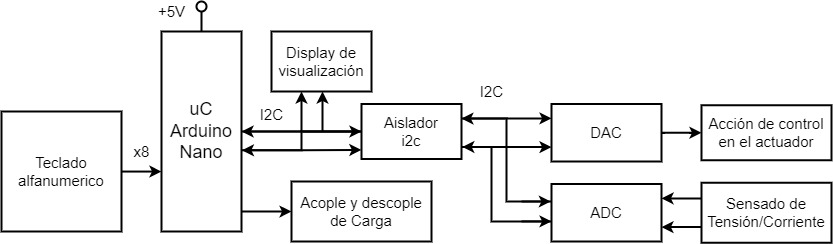
\includegraphics[scale=0.5]{./imagenes/diagrama_digital.jpg}
    \caption{Estructura de archivos de la plantilla.}
    \label{F:diagrama_digital}
\end{figure}

\section{Componentes de la etapa digital.}

\subsection{dsPIC30F4011. High-Performance, 16-Bit Digital Signal Controllers.}
El dsPIC30F4011 es un controlador digital de señales de 16 bits, reconocido por su alto rendimiento y sus amplias capacidades. Diseñado por Microchip Technology, este dispositivo se destaca por su versatilidad, lo que lo convierte en una opción ideal para una variedad de aplicaciones en el ámbito industrial, comercial y de consumo.
Con su arquitectura avanzada y su conjunto completo de características, el dsPIC30F4011 ofrece un rendimiento excepcional en aplicaciones que requieren un control preciso y eficiente de señales digitales. Su capacidad para manejar operaciones complejas en tiempo real lo hace adecuado para una amplia gama de proyectos, desde sistemas de control hasta aplicaciones de procesamiento de señales. Esta también se destaca por su tamaño compacto y su diseño robusto, lo que lo hace fácil de integrar en una variedad de dispositivos y sistemas electrónicos. Además, su amplio rango de temperatura de funcionamiento y su bajo consumo de energía lo hacen adecuado para aplicaciones en entornos exigentes.

\underline{programación}
La programación del dsPIC30F4011 se lleva a cabo utilizando el software MPLAB IDE v8.91, desarrollado por Microchip Technology Incorporated en los Estados Unidos. MPLAB IDE proporciona un entorno de desarrollo integrado (IDE) que facilita la creación, depuración y programación de aplicaciones para microcontroladores de la familia dsPIC.
Este software ofrece una variedad de herramientas y características que simplifican el proceso de desarrollo de software para el dsPIC30F4011, incluyendo un editor de código, compilador, depurador y simulador. Además, MPLAB IDE es compatible con una amplia gama de dispositivos de Microchip, lo que lo convierte en una opción versátil para los desarrolladores de sistemas embebidos.
El código utilizado en el dsPIC30F4011 está disponible en [insertar referencia aquí], que es un enlace a un repositorio en GitHub. Este repositorio contiene el algoritmo desarrollado en los capítulos anteriores, permitiendo a los interesados examinar y comprender el funcionamiento del sistema implementado. La disponibilidad del código fuente en un repositorio público facilita la colaboración, revisión y mejora continua del proyecto, además de proporcionar una referencia para futuros desarrollos y aplicaciones relacionadas con el dsPIC30F4011.

Protocolo de comunicación.
El protocolo de comunicación es fundamental en el diseño y desarrollo de sistemas embebidos, ya que define la manera en que los dispositivos intercambian información entre sí. En el caso del dsPIC30F4011, se cuenta con diversas opciones de protocolos de comunicación, cada uno con sus propias características y aplicaciones específicas.
Entre los protocolos de comunicación compatibles con el dsPIC30F4011 se encuentran:
SPI™ (Serial Peripheral Interface): Permite la comunicación síncrona entre dispositivos mediante una línea de reloj común y líneas separadas para datos de entrada y salida.
I2C™ (Inter-Integrated Circuit): Proporciona una interfaz de comunicación de bus de dos cables que permite la comunicación entre múltiples dispositivos conectados al mismo bus.
Universal Asynchronous Receiver Transmitter (UART): Permite la comunicación serial asíncrona entre el dsPIC30F4011 y otros dispositivos periféricos.
CAN (Controller Area Network): Es un protocolo de comunicación serial diseñado para aplicaciones de control en tiempo real, especialmente en entornos automotrices e industriales.
Para este proyecto en particular, se optará por emplear el protocolo I2C debido a su compatibilidad con los componentes utilizados en la fuente. La elección de este protocolo se fundamenta en su eficiencia y versatilidad, lo que lo hace idóneo para satisfacer los requisitos de comunicación de este sistema embebido.

\begin{figure}[H]
    \centering 
    
\includegraphics[scale=0.5]{./imagenes/mplab.jpg}
    \caption{Logo MPLAB IDE.}
    \label{F:LogoMPLAB}
\end{figure}

\subsection{Teclado de membrana 4x4.}
El teclado de membrana matricial 4x4 autoadhesivo es un dispositivo de entrada que se utiliza comúnmente en aplicaciones electrónicas donde se requiere una interfaz de usuario simple y compacta. Consiste en una delgada lámina de material flexible que contiene una matriz de botones dispuestos en filas y columnas, con un total de 16 botones en este caso particular (4 filas x 4 columnas).
Cada botón en el teclado de membrana está interconectado mediante una disposición de líneas conductoras en la membrana. Estas líneas están organizadas de manera que forman una matriz, permitiendo la detección de la ubicación específica de la tecla presionada. El funcionamiento del teclado de membrana matricial implica un proceso de escaneo continuo de todas las filas y columnas para detectar la presencia de un botón presionado. Cuando un botón se presiona, se cierra un circuito entre la fila y la columna correspondientes, lo que indica al microcontrolador la ubicación de la tecla activada.

\begin{figure}
    \centering [H]
    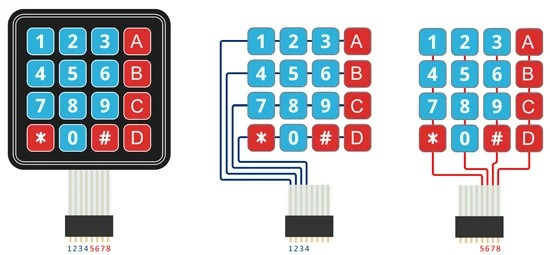
\includegraphics[scale=0.5]{./imagenes/Teclado Matricial 4x4_2.jpg}
    \caption{Estructura de archivos de la plantilla.}
    \label{F:teclado4x4}
\end{figure}

\subsection{Display OLED SSD1306.}
El display OLED SSD1306 elegido para el proyecto utiliza comunicación I2C y ofrece una resolución de 128x64 píxeles. En la Figura 4.13 se presenta una imagen del display, que opera dentro de un rango de voltaje de 3.3 a 5.5 V, lo cual lo hace compatible con el microcontrolador seleccionado. En esta pantalla se mostrará tanto el menú de funcionamiento los modos de operación como un indicador a tiempo real de las magnitudes registradas. Será el vínculo principal entre el usuario y la fuente.

\begin{figure} [H]
    \centering 
    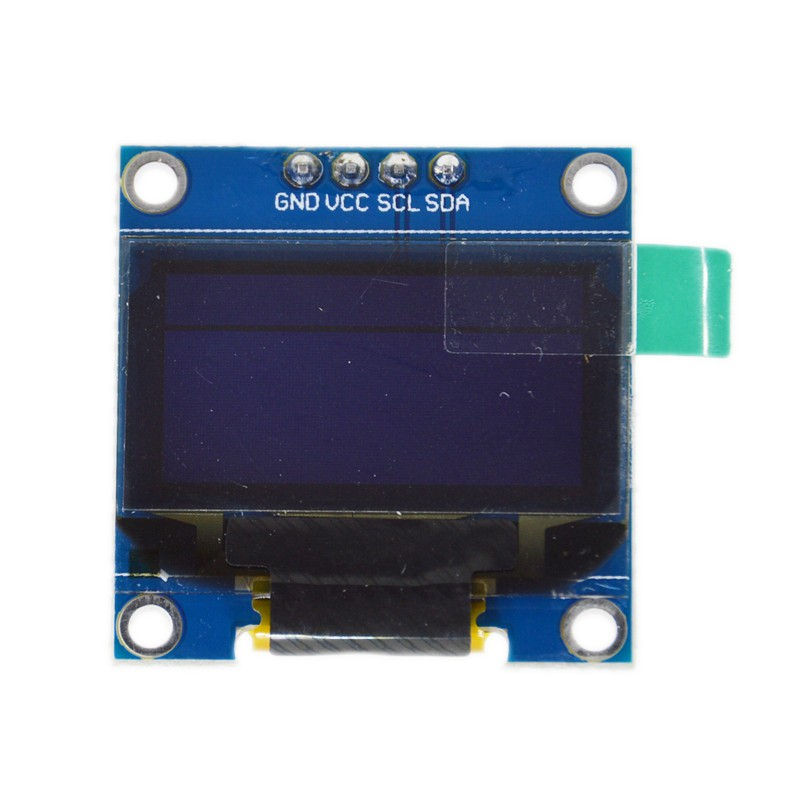
\includegraphics[scale=0.1]{./imagenes/display.jpg}
    \caption{Display OLED SSD1306.}
    \label{F:display}
\end{figure}

\subsection{Aislador I2C capacitivo.}
El dispositivo a utilizar es un ISO1540 [insertar referencia] el cual cuenta con buffers de entrada y salida que están separados por tecnología de aislamiento capacitivo de Texas Instruments que utiliza una barrera de dióxido de silicio (SiO2). Cuando se utilizan con fuentes de alimentación aisladas, estos dispositivos bloquean voltajes altos, aíslan tierras y evitan corrientes de ruido que puedan ingresar a la tierra local e interferir o dañar circuitos sensibles. Esta tecnología de aislamiento ofrece ventajas en función, rendimiento, tamaño y consumo de energía en comparación con los optoacopladores.
De este modo tendremos la aislación galvánica para separar apropiadamente la parte de potencia de la de control.
\begin{figure}[H]
    \centering
    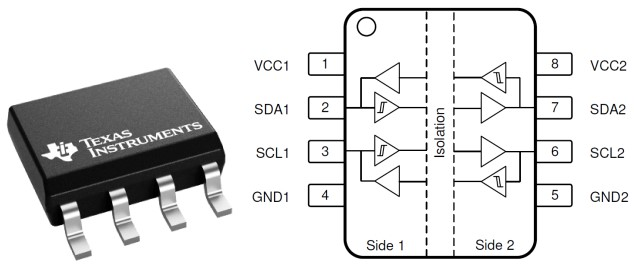
\includegraphics[scale=0.1]{./imagenes/optoi2c.jpg}
    \caption{Aislador capacitivo I2C ISO1540.}
    \label{F:optoi2c}
\end{figure}

\subsection{Convertidor analógico digital. AD.}
El ADS1115 es un componente crucial en la transición de una fuente de alimentación de corriente continua de analógica a digital. Este dispositivo ofrece una impresionante precisión de 16 bits, junto con una velocidad de muestreo de hasta 860 muestras por segundo a través del protocolo de comunicación I2C. Configurable para operar con cuatro canales de entrada de un solo extremo o dos canales diferenciales, el ADS1115 se destaca por su versatilidad en la medición de señales analógicas en entornos digitales. 
Equipado con un conversor delta-sigma de 16 bits, un comparador programable con salida directa al pin de alerta, y una ganancia ajustable que permite la lectura de hasta 256mV en escala completa, este dispositivo garantiza una captura precisa de los datos analógicos. Su interfaz de comunicación I2C facilita la lectura de datos digitales, mientras que su dirección predeterminada de 0x48 y la disponibilidad de bibliotecas para plataformas como Arduino lo convierten en una opción conveniente y de fácil integración en proyectos electrónicos.
\begin{figure}[H]
    \centering
    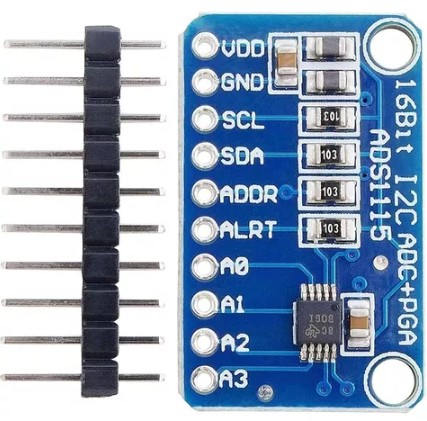
\includegraphics[scale=0.1]{./imagenes/ads1115.jpg}
    \caption{Convertidor AD ADS1115.}
    \label{F:ADC}
\end{figure}

\subsection{Modos de funcionamiento.}
El sistema de control de la fuente de alimentación implementa varios modos de funcionamiento para adaptarse a diversas necesidades de aplicación. A continuación, se describen los principales modos de operación:
Modo Tensión:
En este modo, la fuente de alimentación establece inicialmente el valor máximo de tensión deseado. Posteriormente, limita la corriente máxima de umbral que la carga podrá obtener. Este modo es especialmente útil cuando se requiere controlar la tensión suministrada a la carga de manera precisa y garantizar la seguridad del sistema al limitar la corriente máxima.
Modo Corriente:
En el modo de corriente, la fuente de alimentación establece y controla la corriente suministrada a la carga. Este modo es útil en situaciones donde es crítico mantener la corriente dentro de ciertos límites para proteger los componentes de la carga y garantizar su correcto funcionamiento.
Modo Rampa:
El modo de rampa tiene como objetivo generar un aumento gradual y lineal de la tensión suministrada a la carga durante un período de tiempo determinado. Los parámetros configurables en este modo incluyen la tensión final deseada y el tiempo en el cual se alcanzará esta tensión desde un valor inicial de 0V. Este modo es útil en aplicaciones donde se requiere un inicio suave del sistema para evitar sobrecargas o picos de corriente al arrancar la carga.

